In this section, we describe the move execution layer. This layer is responsible for one of the key functionalities of our project which is the UR5 Robotic Arm's movement, which allows for the checkers game to take place between the user and the co-bot. The move execution layer is made up of three subsystems, the UR5 Robot Arm itself, the electromagnetic gripper, as well as an Arduino.

\subsection{Layer Hardware}
In terms of the Move Execution Layer the most heavily involved hardware component for this layer is the UR5 robotic arm itself. 

\subsection{Layer Operating System}
This layer utilizes Robot Operating System (ROS), although we do not primarily use ROS as we are primarily using Python to move our co-bot. ROS will be utilized to check the status of our robot's arm movements/coordinates at any given time.

\subsection{Layer Software Dependencies}
This layer will also utilize the Python 3.10.6 programming language. 

\begin{figure}[h!]
	\centering
 	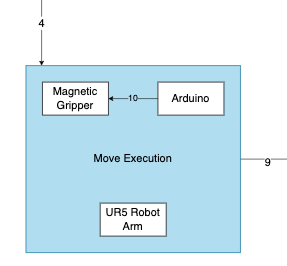
\includegraphics[width=0.60\textwidth]{images/move_execution.png}
 \caption{Move Execution subsystem description diagram}
\end{figure}

\subsection{UR5 Robot Arm}

The UR5 co-bot arm must be able to follow the instructions as asked by the software in order to hover over the correct location on the checker board. The robot must be able to move to fixed locations as predetermined by ROS and our custom software in order to not only move to specified pieces on the board but also to the collection box, and a waiting position.

The UR5 co-bot arm is responsible for the main mechanics of our project. As its ability to move to move to a spot on the board and pick up a piece and move it to another position is necessary so that the UR5 can play against its human oppponent.


\subsubsection{Subsystem Hardware}
In the UR5 Subsystem as well as the Move Execution Layer, the hardware component involved is the UR5 robotic arm itself.

\subsubsection{Subsystem Operating System}
The operating system required here is ROS.

\subsubsection{Subsystem Software Dependencies}
This subsystem layer will require a Universal Robots Python library so that we can control the co-bots movements through python scripts. The Python library we intend on using for this is ur\_rtde.

\subsubsection{Subsystem Programming Languages}
The UR5 subsystem requires the Python 3.10.6 programming language.

\subsubsection{Subsystem Data Structures}
The pre-recorded coordinates of our robot's movements will be saved into a multi-dimensional array so that our robot will have a list of saved positions to go to. The decision on where to go is determined by our Move Decision layer.

\subsubsection{Subsystem Data Processing}
N/A

\subsection{Magnetic Gripper}
The Magenetic subsystem of our Move Execution Layer is responsible for the UR5 robotic arm's ability to "pick-up" each checkers piece. This subsystem is integral to the project as a whole because without it the pieces will not be moved and the checkers game cannot be played.

\subsubsection{Subsystem Hardware}
This subsystem requires more hardware components than some of our other subsystems. It consists of an Arduino, an electromagnet, transistor NPN(2N3904), diode(1N4148), 22K Ω resistor, wires, breadboard, as well as a 3D printed attachement so that it can be screwed into the UR5 arm.

\subsubsection{Subsystem Operating System}
N/A

\subsubsection{Subsystem Software Dependencies}
This subsystem layer requires the Arduino 2.0.3 IDE. As that is needed for us to provide python scripts to Arduino which in turn will power our electromagnet.

\subsubsection{Subsystem Programming Languages}
The UR5 subsystem requires the Python 3.10.6 programming language.

N/A

\subsubsection{Subsystem Data Processing}
N/A